\documentclass[10pt]{article}

% Math formatting
\usepackage{amsmath}
\usepackage{amssymb}

\usepackage{subfigure}

% Lay out packages
\usepackage[margin=4cm]{geometry}
\usepackage[utf8]{inputenc}
%\usepackage{mathpazo}

% Dutch style of paragraph formatting, i.e. no indents. 
\setlength{\parskip}{1.3ex plus 0.2ex minus 0.2ex}
\setlength{\parindent}{0pt}

% Command for Horizontal lines
\newcommand{\HRule}{\rule{\linewidth}{0.5mm}}
% Command for degree symbol
\newcommand{\degree}{\ensuremath{^\circ}}

% Add images and pdf pages
\usepackage{graphicx}
\usepackage{pdfpages}

% Colored rows in tables
\usepackage[table]{xcolor}

% Clickable links with hyperref package
\usepackage[pdfborder={0 0 0 0}, linkcolor=black, urlcolor=blue]{hyperref}

% Fancy Header
\usepackage{fancyhdr}
\pagestyle{fancy}

% Psuedo code
\usepackage{algorithm}
\usepackage{algorithmic}

\rhead{\large\bfseries Assignment 1} % right header: document title
\lhead{\textsc{Jurriaans}, \textsc{Latour} \& \textsc{van der Molen}} % left header: document author
\cfoot{\large \thepage} % center footer: page number

\setlength{\headheight}{18pt}

\begin{document}

\begin{titlepage}
\begin{center}

\includegraphics[width=1\textwidth]{img/uva}\\[1cm]
\HRule \\[0.4cm]
% Title
 Assignment 1\\\small Independent Agents and Multi-Agent Coordination\\[0.4cm]
\HRule \\[1cm]
\begin{tabular*}{0.95\textwidth}{@{\extracolsep{\fill}} l c r}
Robrecht \textsc{Jurriaans} & Sander \textsc{Latour} & Hessel \textsc{van der Molen}\\
\textsc{5887380} & \textsc{5743044} & \textsc{5619785}\\
\end{tabular*}
\\[0.4cm]



\vfill \today
\end{center}
\end{titlepage}

% \newpage
% \thispagestyle{empty}
% \mbox{}
% \pagebreak

% \setcounter{tocdepth}{2}
% \tableofcontents
% \pagebreak


\section{Introduction}\label{introduction}
%\input{introduction}
In this paper we will solve a predator-prey game within the PURSUIT-domain\footnote{http://www.cs.cmu.edu/afs/cs/usr/pstone/public/papers/97MAS-survey/node8.html} where a group of predators have to hunt down a number of prey. The world consists of an $n*m$ grid in which the agents can move either to the four orthogonal squares or to all eight surrounding squares. The world used here is a toroidal world in which the agents can move of the grid and emerge on the other side of the grid as seen in figure \ref{fig_torwor}. The initial condition that needs to be satisfied in order for a predator to capture a prey is that the predator moves to the cell in which the prey is located. 

\begin{figure}[h!tb]
\centering
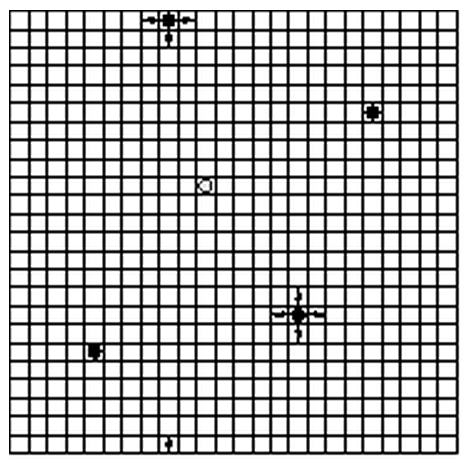
\includegraphics[width=0.6\textwidth]{img/toroidal}
\caption{Orthogonal movement in a toroidal world}
\label{fig_torwor}
\end{figure}

\paragraph{Agent Behavior}
The prey can either move to any unoccupied cell of the four cells located orthogonally around the prey with a probability of $0.8$ or stand still with a probability of $0.2$. The initial behavior of the predator is also random and does not use the information retrieved by the predators sensors.

\paragraph{Overview of Paper}
In section \ref{theory} we will discuss both rational independent agents and basic coordination between multiple agents. In section \ref{application} we will discuss how coordination can be applied to improve efficiency in the predator-prey task. We will then describe our implementation in section \ref{implementation}. Finally we will show the benchmark of our implementation in section \ref{experiments} and draw conclusions from the results in section \ref{conclusion}.


\section{Theory}\label{theory}
% Multi Agent Systems
In a multi agent system it is necessary for each agent to rationally decide on what action all agents will take so that the joint action maximizes the reward. An easy method to accomplish this is to have communication between agents so that all agents can communicate their observations to one agent which then selects the joint action that maximizes the reward and communicates this joint action back to all other agents. If the agents are incapable of communication it becomes important for each agent to rationally derive the action each agent needs to take. It is then important that each agent finds the same joint action. For this to happen it is necessary to have coordination between agents\cite{Vlassis} since it is possible that multiple joint actions maximize the reward. However, if agents select different joint actions it may very well be that the resulting joint action does not maximize the reward.


% Conventions/Roles


\section{Application}\label{application}
In the pursuit domain it is possible to simply use rational independent agents. Various predators each find the closest prey and makes a move which lessens the distance to that prey. The closest prey can be chosen by using the prey with the smallest euclidean distance, but since the agents are only allowed to move orthogonally manhattan distance is a more logical choice. Another possibility is to use a path planning algorithm such as A* to find the actual distance to the prey. Selecting the right action is simply a case of taking the larger of the relative distances of both the x-axis and the y-axis.

% Predators selecting prey
If multiple predators need to surround a prey in order to catch it, coordination becomes very important. If there are multiple prey and predators needs to cooperatively hunt the same prey, it is necessary for each predator to select the same prey to hunt. With communication the predators could simply elect a leader to which they broadcast their closest prey and then the leader selects the prey to attack and communicates this back to the other predators.

However, if communication is not possible the predators are dependent of using their observations to select the same prey based on their independent observations. The first problem is to find the prey closest to all predators. Since the world is toroidal it is impossible to determine this without the knowledge of the size of the world as seen in table \ref{tab_disprob}. Predator 1 sees the prey to its left with a distance of 1 cell, while it sees predator 2 to the right with a distance of 3 cells. If predator 1 does not know the size of the world it will deduct that predator 2 has a distance of 4 cells to the prey. However, predator 2 is only 1 cell removed from the prey and deducts furthermore that predator 1 also has a distance to the prey of 4 cells.

\begin{table}[h!tb]
\centering
	\caption{A 1x5 world in which the distance to a prey is different for each predator}
\label{tab_disprob}
\begin{tabular}{|c|c|c|c|c|}
\hline
	prey & predator 1& & &predator 2 \\
\hline
\end{tabular}
\end{table}

If we do know the size of the world we could find the closest prey, but this gives rise to another problem in which two of the prey have an equal distance to the predators. So now the predators need a convention to select the prey to attack. This would require the predators to have either an order in which it is specified which prey to attack first. Because the observations are in random order it is impossible to know which prey is the first to attack in the hierarchy. To do this it is possible to order the prey based on their combined relative distance. For instance, if the combined distances to prey 1 is 5 cells over the x-axis and prey 2 is -5 cells over the x-axis, which is essentially the same distance, we could simply state that the largest combined distance is the closest. In this case prey 1 is attacked first. If this fails, the same can be done using the y-axis and if this fails then both prey are located in the same cell in which case the joint action that minimizes the distance would be the same for both prey.

% Predators determining which predator needs to occupy which cell
Once a prey has been selected, the predators need to agree on which cell they should occupy. To do this the predators can calculate the distance to each of the four cells for each of the predators and choose the cell that has the smallest distance to the predator. If two predators have the same cell they want to occupy the one with the smallest distance to that cell will ignore this cell and take the second cell which is closest to the predator. This results in the predators to go for the cell which minimizes the total distance of the predators to the cells around the prey. In the case of the same distances between cells or between predators to cells, the same ordering can be used as before over the x- and y-axis. The full algorithm can be found in algorithm \ref{alg_hunt}.

\begin{algorithm}
\caption{Algorithm for determining next action}
\label{alg_hunt}
	\begin{algorithmic}
\REQUIRE $Dprey=\textrm{Distances to each prey}$, $Dpred=\textrm{Distances to each predator}$
\STATE $n=\textrm{Size of world}$
\STATE \COMMENT{For each prey calculate the total distance to all predators}
\FORALL{$Dprey$} 
\STATE $CrtDis=0$
\FORALL{$Dpred$}
\STATE $CrtDis += -(Dpred-Dprey)\mod n$
\ENDFOR
\IF{$CrtDis<MinDis$}
\STATE $MinDis=CrtDis$
\STATE $MinPrey = Dprey$
\ENDIF
\ENDFOR

\STATE \COMMENT{Select closest cell to attack}
\FORALL{Dpred}
% Calculate closest cell for each predator
\STATE Calculate distance to each cell around prey
\IF{two predators have same closest cell}
\STATE predator with smallest distance to cell ignores this cell
\ENDIF
\ENDFOR
\STATE move towards designated cell
\end{algorithmic}
\end{algorithm}

%collision detection
When moving towards its designated cell, a predator may not collide with another predator. This problem is solved by computing the designated cell for each predator and using the current position to move towards this cell. The predator at the largest distance is the predator which moves first. By default each predator tries to decrease the distance on the axe which is the furthest of the prey. Once a movement is done, the next prey pick a move. If this move collides with a move done by another predator, the current predator picks a move with a ``higher rank": a move which is less preferable. In total there are 5 possible moves for a predator. Each move with its corresponding ranking is displayed in table \ref{tab_moveRank}.

\begin{table}[h!tb]
\centering
	\caption{Ranking of possible moves of a predator}
\label{tab_moveRank}
\begin{tabular}{c|c}
Move 							& Rank \\ \hline
Move along longest axe towards prey	& 0 \\
Move along shortest axe towards prey	& 1 \\
Do not move						& 2 \\
Move along shortest axe away from prey	& 3 \\
Move along longest axe away from prey	& 4
\end{tabular}
\end{table}

%surrounding a prey with 3 predators.
During the pursuit, it very likely that 3 predators surround a prey, while the fourth predator is directly behind these predators. Since the prey walks with a 80 percent change towards an unoccupied cell, it becomes hard to catch the prey: the predators will continue to pursuit while not able to move past the prey. In this case the forth predator should walk in the opposite direction, which results (due to the toroidal world) in a capture from the other side. When such a situation is detected, the movement of the fourth predator is overruled.


\section{Implementation}\label{implementation}
% Manhattan distance prey
Since predators can only move orthogonally the best distance to take is the manhattan distance which is a summation of the x distance and the y distance. If predators were allowed to move to the four diagonal cells it would be better to use euclidean distance. 

Each predator uses the observation to create matrices that hold information about the distances of the predators to each prey. These are used to derive which prey is closest by using algorithm \ref{alg_hunt}. The distances of the predators to the prey that has the smallest average distance to the predators is then split into the distances to the four surrounding cells of the prey. This results in a 4 by 4 matrix in which the manhattan distance of each of the four predators to each of the four cells is contained. This matrix is then used to derive the best cell for each predator to go to. This is done iteratively because it is possible that two of the other predators want to attack the same cell so that one of them is forced to another cell which could be the same cell that the predator wanted to attack. For each predator the closest cell is calculated, if two predators have the same cell they want to attack the distance to that cell is set to infinite for the predator that was closest to that cell. The algorithm is then repeated so that the predator ignores that cell.

\section{Experiments and results}\label{experiments}
\subsection{Rational Independent Agents}
If there are two predators and one prey and the predators move randomly, than the average capture time after 10 episodes is $242.22$ cycles. If we use the observation of the prey we can easily increase this to an average of $9.24$ cycles after 500 episodes (and a deviation of 5.6). This increase was to be expected since at each step the predators try to minimize the distance to the prey. When there are two prey the average cycles increases to $14.14$ after 100 episodes. 


\subsection{Multi-Agent Coordination}
Using 4 predators, which needs to completely surround 1 prey, and 2 prey, our implementation has an average capture time of 32.7 cycles per episode (based on 500 episodes) and a deviation of 41.0. Due to some (near) infinite loops in the system, some episode end in 100+ cycles. Therefore the deviation is quite large.\\
In theory, the problem could also be solved with the use of A* (with an action set for each agent of  actions). This approach would result is the most optimal path for each agent, and therefore in one of the most optimal  solutions to catch the prey. However, when implemented the system got to a hold, meaning that solving the problem with A* is a too expensive task.


\section{Conclusion}\label{conclusion}
%\input{conclusion}
Our implementation has a few shortcomings. The first is that it is possible to enter an infinite loop. An example of a world which results in an infinite loop is shown in table \ref{tab_loop}. All mirrored and rotated versions of this world also results in an infinite loop. The exact reason why this happens is yet unknown, but it probably can be solved by adjusting the collision detection. Another solution to solve the loop would be to introduce a random move when a pursuit takes longer than $x$ cycles. Despite a collision detection, the systems sometimes encounters a collision. We also weren't able to trace the origin of the problem: prey selection, collision detection and cell-assignment all work in the way we thought it should work. 

\begin{table}[h!tb]
\centering
	\caption{A 4x5 with a loop}
\label{tab_loop}
\begin{tabular}{|c|c|c|c|c|}\hline
	 &  & & & \\ \hline
	 & prey & pred & pred & \\ \hline
	 & pred & pred & & \\ \hline
	 &  & & & \\ \hline
\end{tabular}
\end{table}



% References
 \pagebreak

 \bibliographystyle{plain} % plain, nature, jbact
 \bibliography{myref} 
 
 \pagebreak
 \appendix
 %\input{appendix}

\end{document}
